\chapter{Analysis of the social network \Twitter}
\label{chapter:analysis}

The work now wants to take a closer look at a concrete social network.
There are of course many social networks, which can be used for harvesting
data, however, as a case study, the work wants to concentrate on a big social
network, which is widely used by employees and individuals. Moreover,
an \textit{API} is needed to gather data automatically.

As a case study the choice was between \textit{Facebook} and
\Twitter. Both are widely used, however \Twitter{} was chosen due to many
already existing programs and platform bindings. Furthermore \Twitter{} is
somewhat more dynamic than \textit{Facebook}, as it offers the possibility to
parse \Twitter{} messages and not just handling static data.

\Twitter{} is a popular social networking and micro-blogging service, that
enables users to post messages and to let other users follow those messages.
The term \textit{micro-blogging} describes a form of communication, that
consists of brief messages in text form, which then can be send over a variety
of ways, like instant messages, mobile phones, e-mail or other \cite{java2007}.

\begin{figure}[hbt]
  \centering
  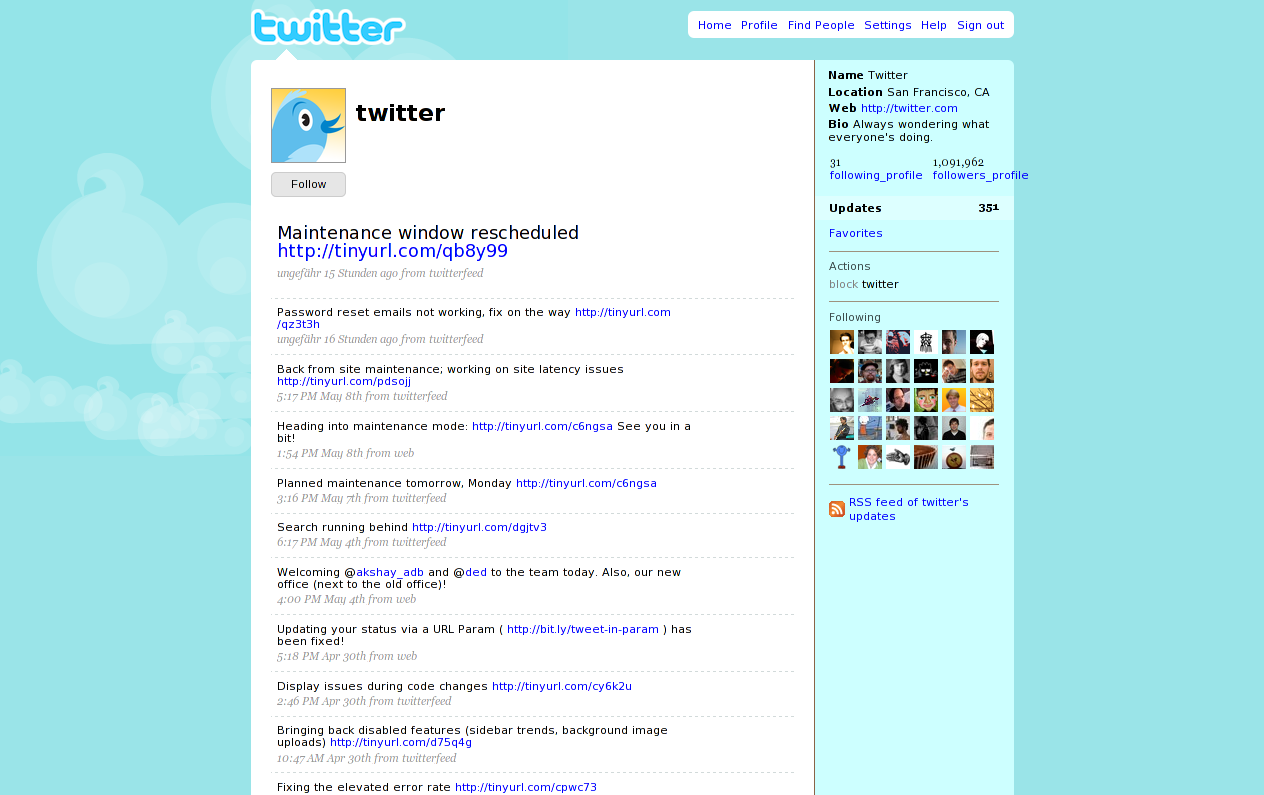
\includegraphics[width=\textwidth]{twitter_screenshot}
  \caption{An example Twitter Homepage, featuring several \Twitter{}
  messages, account information and the users this account
  follows.}\label{fig:twitter_screenshot}
\end{figure}

Micro-blogging itself is relatively new, though already widely used and
provided by services like
\textit{Twitter}\footnote{http://www.twitter.com},
\textit{identi.ca}\footnote{http://identi.ca},
\textit{Jaiku}\footnote{http://www.jaiku.com} and others. \Twitter{} is one of
the most popular micro-blogging services \cite{java2007} and currently
exhibiting more than a million users. The accurate number unfortunately is not
available, however \cite{krishnamurthy2008} estimated about 1.4 million users
in 2008 and \cite{whitworth2009} calculated more than 1.78 million users in
2009.

\Twitter{} limits the length of the messages to 140 characters. The messages
are called \textit{updates} or \textit{tweets}.  The scopes of those messages
range from events, news, daily life and other interests \cite{java2007}. Of
course, other services like Instant Messaging also offers a way to communicate
the such informations, however micro-blogging allows to do this publicly.

As \cite{java2007} describes, micro-blogging is a faster way to communicate
compared to other means of communication, like blogging. It requires less time
to think and write a message, and this of course implements much quicker
\flqq{}write rate\frqq{}. This is of course one of the main differences
between blogging and micro-blogging, whereas an author spends several minutes
to hours to think up and write a blog post. As it now takes less time to think
and write a message, the frequency one can write such, increases and a
micro-blogger may posts several messages a day.

Users may choose to make their messages visible to all users (even those not
logged into \Twitter{}) or to just make them available to \textit{friends}. A
\textit{friend} is a relation inside the \Twitter{} platform, and allows a user
to \textit{follow} the messages from other members, who are added as a
\textit{friend}. Users, who are not a friend to another user can still follow
the user, who they are not friend with, but are then called \textit{follower}.
The friend relation is not forced to be mutual, but can be single-way too. In
addition, a user can choose to make his messages public or just available to
his friends. If the messages are marked as public, they will be displayed in
the public timeline, which can be accessed by the URL
\url{http://twitter.com/public_timeline}.

\cite{java2007} has found, that the types of user interactions are daily
chatter, conversations, sharing informations and reporting news. This of course
leads us to question, which information can be dangerous and which can be used
by a social engineer.

\begin{figure}[hbt]
  \centering
  \begin{tikzpicture}[scale=0.75, transform shape,
                      root concept/.append style={concept color=skyblue1},
                      level 1 concept/.append style={concept color=chameleon2},
                      text=white, mindmap]

    \tikzstyle{every annotation}=[fill=skyblue3, font=\sf]

    \node[concept] (Twitter) {Twitter}
      child[concept, grow=160] {node [concept] {Web Interface}}
      child[concept, grow=125] {node [concept] {Twitter API}
      child[concept, grow=left] {node [concept] {User Applications}}}
      child[concept, grow=90] {node [concept] {Facebook}}
      child[concept, grow=55] {node [concept] {IM}}
      child[concept, grow=20] {node [concept] {SMS}}
      %
      child[concept, grow=200] {node [concept] {Web Interface}}
      child[concept, grow=235] {node [concept] {Twitter API}
      child[concept, grow=170] {node [concept] {RSS}}
      child[concept, grow=210] {node [concept] {User Applications}}}
      child[concept, grow=270] {node [concept] {Facebook}}
      child[concept, grow=305] {node [concept] {IM}}
      child[concept, grow=340] {node [concept] {SMS}};

    \node[annotation] at (52.5:7.5) {Twitter Input Methods};
    \node[annotation] at (307.5:7.5) {Twitter Output Methods};

    \draw (2,0) -- (6,0);
    \draw (-2,0) -- (-6,0);

  \end{tikzpicture}
  \caption{\Twitter{} input and output methods, on the basis of \cite{krishnamurthy2008}.}
  \label{fig:twitter_io}
\end{figure}

A sample \Twitter{} profile page is shown in Figure
\ref{fig:twitter_screenshot}. It features several elements, which we will
discuss in the next section. 

\Twitter{} messages can be sent and received by a variety of methods, all
listed in Figure \ref{fig:twitter_io}. Several of those are or were
discontinued for a certain amount of time, but either re-enabled or provided by
a third party company.


\section{Methodology}

In this work, a five-step approach was used to characterize useful information,
extraction and countermeasures. The target was to define the steps needed for
executing an attack like already described.

\begin{enumerate}
\item Data was obtained from the \Twitter{} social network from several users.
The data was taken from famous persons on the network, as well as less famous.
Furthermore users, who were very active as well as less active users were
watched.
\item The data gathered in the first step was studied and it was determined, which
attacks are possible. 
\item Three sample attacks, which happened for real in the last years, were
chosen. All of these attacks are described by \cite{mitnick2003}. The chosen
attacks were then transfered to the
prototype and the \Twitter{} social network.
\item The attacks were tested on sample profiles for their feasibility and efficiency
\item Countermeasures were elaborated to mitigate the risk of such attacks.
\end{enumerate}


\section{\Twitter{} profile data}
\label{sec:twitter_profile_data}

As already mentioned, a \Twitter{} profile page consists of a series of
elements, which can be used for harvesting data. We now want to take a closer
look at those elements, the content and how a social engineer can extract data
out of those fields.

\begin{description}
\item[Name] This fields tells the real name of a user, it is limited to 20
            characters. It is required to enter a name, albeit a bogus name is
            also accepted. The field is required.\\
            \textit{Example: Peter Sample}
\item[Username] The username is presented with this field. A username is needed
                to create an URL, which is of the form \url{http://www.twitter.com/[username]}.
                Therefore only letters, numbers and underscore are allowed. The maximum length
                is set to 15 characters. The field is required.\\
                \textit{Example: petersample}
\item[User ID] The user id which is handed out automatically. The sequence is
               not known, however it is mostly agreed, that the user id is not given out
               sequentially.\\
               \textit{Example: 1234567}
\item[E-mail] Though not visible publicly, a \Twitter{} user has to provide an
              e-mail address. As described by \cite{brown2008}, though not provided an e-mail
              address can be build out of a naming scheme and the already
              given data, like the username and the real name. If the user
              is an employee of a certain company, this might be even easier,
              as companies often have certain naming schemes. The field is required.\\
              \textit{Example: petersample@example.com}
\item[More Info URL] The URL is used to link a visitor of a profile to further
                     websites, like the blog of the owner. It can link to
                     any site on the internet. The shown component of the
                     URL is 17 characters. Except XSS prevention,
                     \Twitter{} does not rewrite of the URL, and port numbers
                     after the TLD, spaces, German umlauts and UTF-8 characters were
                     accepted.\\
                     \textit{Example:} \url{http://www.petersample.com/},\\
                     \texttt{http://www.peter sample.com:8080/äöü$\Gamma\Lambda\Sigma\Psi$.htm}
\item[One Line Bio] A short sentence can be shown on the profile page, where a
                    user can describe himself. It it limited to 160
                    characters.\\
                    \textit{Example: I am a computer science expert and work
                    for example.com}
\item[Location] The location will also be shown on the profile page and is
                limited to 30 characters.\\
                \textit{Example: Munich}
\item[Picture] A user can insert a picture of himself, although it is not
               required to do so. Moreover, if a user publishes an image, it does not have to
               show himself, but can also be anything else.
\item[Profile Creation date] The date, the profile was created.\\
              \textit{Example: Fri Nov 02 00:17:11 +0000 2007}
\item[Following] Describes a list of users, the profile owner is \textit{following}.
                 To see the list, one has to be logged in.
\item[Followers] This gives us a list of users on the \Twitter{} network, who
                 are \textit{following} the profile owner. To see the list, one has to be logged in.
\item[Friends] This are users, who have a bidirectional connection. That means,
               that user A is following user B and vice versa.
\item[Favorites] A user can mark his messages or the messages from other users as
                 a favorite, which displays a
                 yellow star beneath them. A users favorite messages can be viewed
                 by visiting \url{http://twitter.com/favorites?user=[username]}.
\item[Messages] Finally the messages, which are composed by the actual message,
                which is limited to 140 characters, the time, when the message
                was written and by which mean. A message is identified by a unique
                id, e.g. 1767572233 and can be accessed by
                \url{http://twitter.com/[username]/status/[message id]}.

                \Twitter{} also offers special commands, which can enhance a
                message or turn a \Twitter{} into a query tool.
  \begin{description}
    \item[@username + message]
      A message can be sent directly to another person, though still visible
      publicly.\\
      \textit{Example: @petersample yes, you are totally right!}

    \item[D username + message]
      In contrast to the command above, this message is entirely private and
      not visible by other users.\\
      \textit{Example: D petersample this is a private message for peter!}

    \item[WHOIS username]
      retrieves information of any public user on the \Twitter{} platform.
      Currently, this command returns the real name, the date since the user
      has an account on \Twitter{}, the one line bio, the website and the
      location.\\
      \textit{Example: WHOIS petersample}\\
      \textit{Answer: Peter Sample, since May 2009. bio: I am a computer
              science expert and work for example.com. location: Munich web:
              \url{http://www.petersample.com/}}

    \item[GET username]
      gets the last message this user posted.\\
      \textit{Example: GET petersample}\\
      \textit{Answer: petersample: This is my latest message (1 day ago)}

    \item[NUDGE username]
      sends a note to the user, reminding him to post a message.\\
      \textit{Example: NUDGE petersample}\\
      \textit{Answer (sent to petersample): You've been nudged! [my-username] wants to know what you're doing. Reply to this
      message to update your Twitter friends.}

    \item[FAV username]
      marks the last message of username as a favorite\\
      \textit{Example: FAV petersample}

    \item[STATS]
      returns the number of followers and how many users the account itself is
      following.\\
      \textit{Example: STATS}\\
      \textit{Answer: followers: 135 following: 47}

    \item[INVITE phone number]
      sends an invite SMS to the phone number\\
      \textit{Example: INVITE 123 456 7890}

\end{description}
\end{description}



\section{Message classification}

\cite{java2007} described a classification of the messages on the \Twitter{}
platform. After they gained a dataset, the author and his team tried to
categorize each message. The results were the following:

\begin{description}

\item[Daily Chatter]
Most users on \Twitter{} post about what they are currently doing or similar
things. Of course, they are answering the question \flqq{}What are you
doing?\frqq{}, which can be found over the input field of a message. This is
the most common use of the \Twitter{} platform.

\item[Conversations]
There are two ways to communicate with another user, one is by public
messaging, which features the @ symbol like stated above, the other one is
private messaging, which uses the D character. \cite{java2007} discovered, that
about one eighth of all posts in their dataset contained a public conversation
and about 21\% of the users in their dataset used this type of messaging. Of
course, there is no data available about private messages.

\item[Reporting news]
Another big piece of the cake is done by users, who report or comment news and
events. Some of them are automated and post weather reports, other are
eyewitnesses and report and event in their location.

\item[Sharing information/URLs]
Many users also share information and websites, and therefore uses services,
like \textit{TinyURL}\footnote{\url{http://tinyurl.com/}} or
\textit{tr.im}\footnote{\url{http://tr.im/}}. According to \cite{java2007},
about 13\% of all posts in the dataset contain at least one URL.

\end{description}


\section{Threats and risks}

All of the above mentioned fields, but of course also the \textit{tweets}
themselves create a threat against the user himself, but also to other users,
who are in contact with him. Even with at first glance useless information,
information about the user can be extracted. For example, if he shares his
location and what he is doing job-wise, his workplace and position can be
easily found. The prototype, which is described in the next chapter, will make
use of exposed data, building a fact sheet about the user and people, who are
in contact with.

\section{Relevant data and the security risks of those at individuals and companies}

\subsection{The challenge of extracting data automatically}

The \Twitter{} social network gives access to a \textit{REST} API, which can be
used by calling either \url{twitter.com} or \textit{search.twitter.com}. The
first one is used for account settings and methods, posting updates and several
other things related to users, their relationship and updates. The latter one
is entirely used for searching for certain updates of users or users
themselves. The API supports \textit{JSON}, \textit{XML}, \textit{RSS},
\textit{Atom} as output formats, allthough just \textit{JSON} is supported on
every API method.

Most API methods require a username and a password, however this is not a
problem by itself, as a \Twitter{} account can be created within minutes by
using a mail address. The real challenge however is the limit of 150 API calls
per hour. If a user is logged in, the user has 150 calls, which he can use on
API calls. If the user is not logged in, i.e. an anonymous user, the IP address
is used for tracking this user. To make use of a very deep information
visualisation of a user, 150 calls are not enough, as for example many users
have more than 150 friends. However, there are three ways around this problem:
The first one is to just use the important data, leaving a deep information
visualisation of e.g. friends aside, the second is to create many accounts, and
then change the accounts during acquiring the data, and the last one to not log
in into \Twitter{} and acquiring the data anonymously, while changing the IP
address after 150 calls. However, some API methods require the user to be
logged in.

\subsection{Ontology and classification of the data}

The \Twitter{} API offers a wide range of methods, however in the first place,
the attacker is mostly interested in gaining information and not that much in
using the API methods to do actions. Additionally the attacker is mostly
interested in a certain person or group, therefore just the methods, which
allow gathering data about a certain user or group makes sense here. For a
social engineering attack, the following data might be interesting.

\subsubsection{General data about the user}
\Twitter{} offers some static fields, which can be altered by the user and
remains mostly the same over the year. Some other information is created
automatically and still accessible by other users.

Most of the fields described in chapter \ref{sec:twitter_profile_data} are
already usable for gaining an already penetrative overview of a person.

\begin{description}
\item[Name] Gives the real name of the user, which can be used for
phishing mails or social engineering attacks, where a name is needed.

\item[Username] Many users use the same username on different
services, like email or other social services. This can be used for some
attacks.

\item[Description] This description might be useful for gathering other useful
information, such as workplace or interests.

\item[Homepage] A personal homepage might give additional
information about the user.

\item[Image] Gives an idea, how the person might
look like.

\item[User ID] Not relevant.

\item[Time Zone] Gives an idea, where the person
lives or works.

\item[Location] Together with the Time Zone, an attacker now
could actually define his work place and home more precise.

\item[Profile Creation date] Tells the attacker
since when the user is using \Twitter{}. That might be a good indication,
whether he also uses other services and since when.

\item[Messages] The Message count could tell how active a person using a
computer or how interested he is in a certain topic.

\item[Followers] An interpretation of the followers count may say how
famous he is and how much effect he could have on other people.

\item[Friends] While the number of friends is not that interesting,
the friends can be used for attacks too, as most of them are real friends
or colleagues.
\end{description}

\subsubsection{Mail addresses}

As already described earlier, the mail addresses of the users are not visible
throughout \Twitter{}, though the addresses can be gathered in most cases.
\cite{brown2008} for example described, that a mail address can be constructed
out of a naming scheme of given data, like the username or the real name.
Another possibility is to look through the messages for anything that looks
like a mail address. Quite often users write messages, about contacting them at
a special address or that they changed to a new one.

\subsubsection{Times}

An analysis of the time of writing messages can be a good instrument to track
down working hours and working days or periods the user is using a computer.
Additionally hours, the user is not available can be tracked too, for example
when the user is doing holidays.

\subsubsection{Replies and friends}

\Twitter{} by itself does not publish the friends of a user, however it
promotes followers and users who follow the candidate. With this data however,
the \textit{hidden} network can be found, which basically is a graph, which
only consists of bidirectional connections. This is the network, the user is
actually friend with. By analysing the replies of messages, it can be found,
with which of the friends, the user has most contact with. This shows then a
quite good representation of the users friends and or colleagues.

\subsubsection{Input sources}

The \Twitter{} input sources give an overview, what methods the user uses to
post updates. For example, if he is using a \Twitter{} client, that is only
available for a certain operating system, this could be exploited. If the
source is mostly SMS, the location is getting even more important, as location
tracking could be done in this case. Also there could be a relation between the
input method and the computer experience the user has, if he is using external
clients or not.

\subsubsection{Interests}

In most messages, the users represent a certain interest in a single topic.
This is either done by marking the topic explicitly with a hash sign or by just
using text to describe the interest. 

\subsubsection{Locations}

Also, many messages include information about the current location, for example
if they arrive at the workplace, at conferences or other. This data can be
filtered by analysing the messages. A promising project, that could be used
here is \textit{TwitterData}\footnote{\url{http://twitterdata.org/}}, which
marks keywords as key value pairs and actually promotes keys like
\textit{location}, \textit{lat} and \textit{long} for location, latitude and longitude
positions.

\subsubsection{Text search}

Finally a text search can be used to get further information about a certain
topic the user wrote about. 

\section{Countermeasures}

The nature of a social network, especially \Twitter{} is sharing data.
Therefore it difficult to encounter attacks. As \cite{brown2008} describes,
there has to be a trade-off between utility and security. Given also, that most
data comes out of analysing the messages, there are not many ways to minimize
the risk.

The first way to minimize the risk, would be to mark the profile as closed for
anonymous users. However, this can be circumvented easily by following the
user.

Another, possibly extreme, way would be to not publish sensitive information
about the user himself, his workplace, friends and other. As this would be
quite hard to accomplish, still lots of information would be easily accessible,
like the times analysis.

Having a look on the whole social network, \Twitter{} might require to be
logged in while viewing the messages of other users. However, an account can be
easily made and so there won't be any surplus.

At last, the social network could limit the API calls and track them more
precise, so that an automatic extraction is no more possible or at least made
harder. This is probably the only countermeasure, which really would hinder an
attacker of gaining information.
